\documentclass[a4paper,12pt,Times New Roman,numbered,print,index]
{report}
\usepackage[utf8]{inputenc}
\usepackage{subcaption}
\usepackage{sectsty}
\usepackage{amssymb} 
\usepackage{longtable}
\usepackage{booktabs}
\usepackage{ltxtable}
\usepackage{hyperref}
\usepackage{amsmath}
\usepackage{graphicx}
\usepackage{placeins}
\usepackage{needspace}
\usepackage[english]{babel}
\usepackage{algorithm}
\usepackage[noend]{algpseudocode}
\usepackage{rotating}
\usepackage{float}
\usepackage{tabto}
\usepackage[a4paper,top=1in,left=1.5in,bottom=1in,right=1in]{geometry}
\chapterfont{\centering}

\newcommand{\sign}[1]{%      
  \begin{tabular}[t]{@{}l@{}}
  \makebox[1.5in]{\dotfill}\\
  \strut#1\strut
  \end{tabular}%
}
\newcommand{\Date}{%
  \begin{tabular}[t]{@{}p{1.5in}@{}}
  \\[-2ex]
  \strut Date: \dotfill\strut
  \end{tabular}%
}

\begin{document}
\begin{center}
	\vspace{12pt}
	\begin{LARGE}
		\textbf{Real time Indoor and Outdoor Positioning system}
	\end{LARGE}
	\vspace{60pt}
	\begin{figure}[h]
		\centering
		
\includegraphics[height = 4cm, width =4cm]{Image/kmitl.png}
	\end{figure}
	\vspace{84pt}
	\begin{Large}
		\\Tanakorn Sanikawatee\\
		Wunwanach Yarn-arph\\
		Sivut Mekareeya\\
	\end{Large}
	\vspace{96pt}
	\begin{Large}
		Bachelor of Engineering in Software Engineering\\
		International College\\
		King Mongkut's Institute of Technology Ladkrabang\\
		Academic Year 2018\\
        		KMITL-201X-IC-B-003-XXX\\
	\end{Large}
	\vspace{12pt}
\thispagestyle{empty}
\end{center}

\begin{titlepage}

\vspace*{\fill}\par

\begin{table}[H]
\begin{tabular}{l}
	{COPYRIGHT 2018} \\
	{INTERNATIONAL COLLEGE} \\ 
	{KING MONGKUT’S INSTITUTE OF TECHNOLOGY LADKRABANG} \\ 
\end{tabular}
\end{table}
\end{titlepage}

\cleardoublepage

\begin{flushleft}
\vspace{24pt}
\par \textbf{{\normalsize Thesis - Academic Year 2018}}\newline
\noindent\par Bachelor of Engineering in Software Engineering
\noindent\par International College
\noindent\par King Mongkut's Institute of Technology Ladkrabang
\newline
\noindent\par \textbf{Title:} Real time Indoor and Outdoor Positioning System \\ \hspace{1.2cm}  
\newline
\noindent\par \textbf{\normalsize Authors:}
\begin{enumerate}
	\item Tanakorn \tabto{3cm}{Sanikawatee} \tab{Student ID: 58090018}
	\item Wunwanach  \tabto{3cm}{Yarn-Arpha} \tab{Student ID: 58090034  }
	\item Sivut \tabto{3cm}{Mekareeya} \tab{Student ID: 58090042  }
\end{enumerate}
\hfill\newline
\hfill\newline
\hfill\newline
\hfill\newline
\hfill\newline
\hfill\newline
\hfill\newline
\hfill\newline
\hfill\newline
\hfill\newline
\begin{table}[h]
	\begin{flushright}
		\begin{tabular}{c}
		Approved for Submission									\\
														\\
														\\
														\\
														\\
		...............................................							\\
														\\
		(Dr. Isara Anantarasilp)								\\
		Advisor											\\
														\\
		Date ......../......../........								\\
		\end{tabular}
	\end{flushright}
\end{table}
\thispagestyle{empty}
\end{flushleft}
\newgeometry{top=2in,left=1.5in,bottom=1in,right=1in}
\section*{\LARGE \centering Abstract}
\vspace{20pt}

\paragraph{}Real-time Indoor and Outdoor positioning system has long been researched and developed. The Global Positioning System (GPS) can locate the object in an outdoor environment, though, it fails to identify the location when the object is inside the building. Thus, there is a need for another technology and system to accomplish the indoor positioning. However, there are still multiple challenges concerning this indoor positioning technology due to environmental factors, such as building structure, which can hinder the signal. Moreover, the noises in Received Signal Strength Indicator (RSSI) also lead to an inaccuracy in positioning. Hence, in this research, we propose a real time indoor and outdoor positioning system using Bluetooth Low Energy (BLE) and GPS technology, and a method to improve the accuracy of indoor positioning by predicting the $n$ (environment variable) which is a variable in Pathloss equation that directly affect the accuracy of object position estimation. 
\thispagestyle{empty}
%Table of Contents and Beginning Documents
\clearpage\phantomsection
\renewcommand*\contentsname{Table of contents}
%\addcontentsline{toc}{section}{Contents}
\tableofcontents
\cleardoublepage
\clearpage\phantomsection

\chapter{Introduction}
\section{Motivation}
\paragraph{}The interest in positioning system has been around for many years, especially after the success of Global Positioning System based on the Global Navigation Satellite Systems (GNSS) technology that enable the outdoor positioning with less than one meter deviation in accuracy [22]. With the achievement of GPS, the next issue to be focused on is the indoor positioning. There has been some proposed approach for indoor positioning such as fingerprinting, triangulation, trilateration, etc. However, the we believed that there is still room for improvement in terms of accuracy for indoor positioning which will complement the full positioning (indoor and outdoor) system along with the use of GPS to achieve the outdoor positioning.
Our thesis proposed a real-time indoor and outdoor positioning system with an improvement in accuracy of Bluetooth Low Energy (BLE)-based indoor positioning. The aforementioned positioning system tends to result in low accuracy positioning due to BLE nature of low power consumption and the fact that other surrounding signals such as WiFi [23] and environmental factors can cause an error in signal strength measurement. Therefore, we believed that by knowing the equation of environment variable during the process of distance estimation will help improve the accuracy.



\section{Problem Descriptions}
\paragraph{}The GPS can only achieve the outdoor positioning due to its limitation. Therefore, there is the need of another technology to implement the indoor positioning. However, the BLE also have problem with accuracy when there is an obstacle or signal interference, making the target object position estimation deviate from the actual target object position.


\section{Objectives}
\paragraph{}The objective of this thesis is to research a method that can enhance the performance of indoor positioning accuracy based on device context information and showcase the visualization of the results real-time on 2-D map in smart phone device. This thesis aims to find the optimal method approach for indoor localization and provide solution for deployment. Our indoor positioning demonstration will be displayed in a 2-D map of a specified floor.
    \begin{itemize}
    	\item Explore the techniques that can improve the accuracy of BLE-based indoor positioning.
    	\item Mobile Application to show the result of indoor positioning by BLE and outdoor positioning by GPS.
    \end{itemize}


\section{Scope of work}
\paragraph{} The scope of our project regarding indoor positioning only applies to an unobstructed or free space environment and the accuracy improvement methods we propose are for BLE-based indoor positioning. Our indoor positioning  system provides a 2-D position of the target.


        	        	 


\chapter{Related Work}
\paragraph{}There are various kinds of studies and researches that are related to this project. This mainly involve Bluetooth Low Energy.

\section{Similar to our proposal}
\paragraph{} There have been multiple proposed methods and multiple technologies for indoors localization. However, most of them use the Bluetooth low energy (BLE) and WiFi technology in the research. Moreover, the Received Signal Strength (RSSI) is one of the most popular and common way to estimate the position. Thus, in this chapter, we present the related work that use BLE and RSSI with these techniques: solely RSSI in distance estimation, Triangulation, Fingerprint-based method, and Trilateration.


Received signal strength indicator (RSSI) is used to estimate the indoor position in \cite{ref:r10}. The observation in this research is done in a 10.5 meters x 15.6 meters room with 22 beacons installed around the room. The system determines the location by measuring which beacon has the highest RSSI value. The experiment achieved the correct estimation rate of 96.6 percent.

In [11], the authors introduced the three-dimensional positioning system using three-dimensional coordinates triangulation to calculate the position of each node and RSSI to measure the distance among beacons. The error rate from estimation is reduced by 27 percent from existed two-dimensional positioning system. 

Fingerprint-based method is another technique used in positioning system. In [12], the authors explored the use of BLE beacons for fingerprint positioning. The research was conducted using 19 beacons distributed around the approximately 600 square meters room. They achieve the tracking accuracies with 95 percent of the time containing an error less than 2.6 meters using dense beacon distribution (one beacon per 30 square meters) and less than 4.8 meters for lower density distribution (one beacon per 100 square meters) compared to the accuracy of error less than 8.5 meters achieved from the WiFi technology using the same method in the same environment.

In [13], the authors presented two post-processing filters (accuracy function and correction function) after applying the trilateration method to enhance the estimated result. The mean and standard deviation of the estimation are minimized after the post-processing filters are added, thus, they concluded that the trilateration method can be used in indoors localization and the post-processing filters are recommended to make the estimation more accurate.

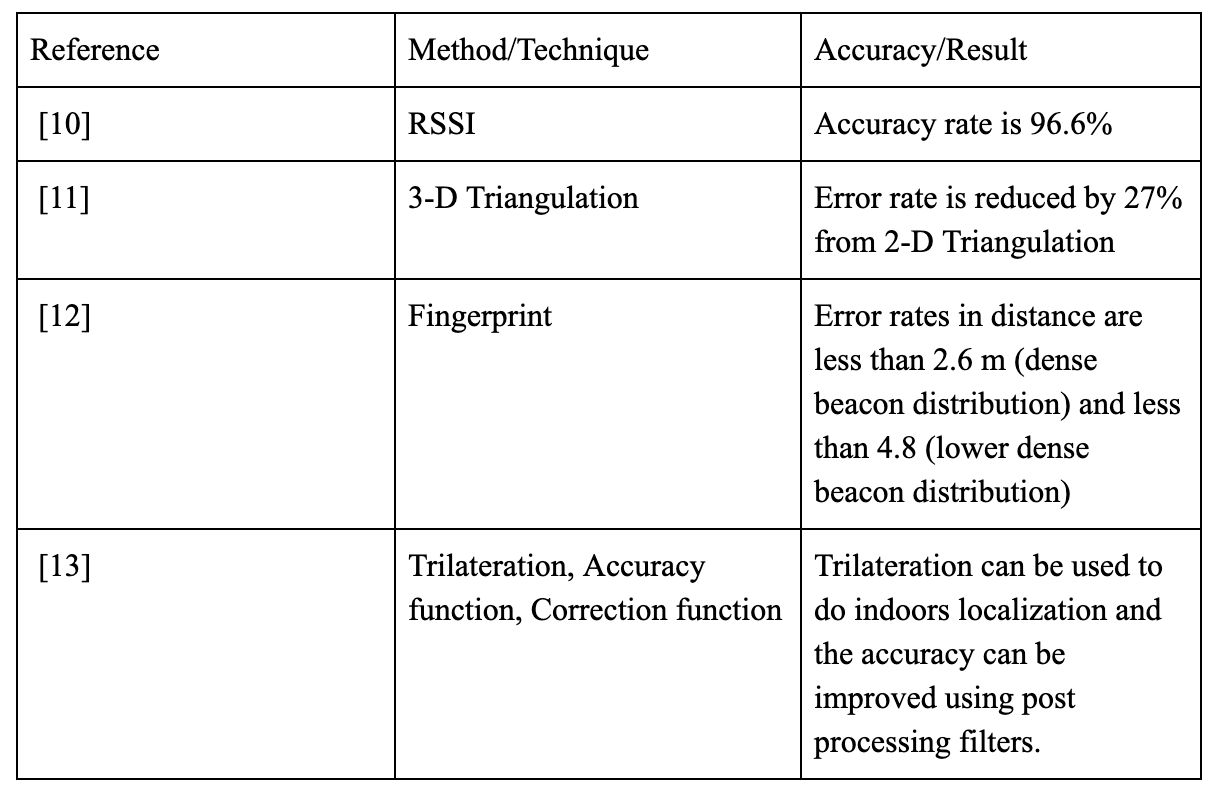
\includegraphics[scale = 0.6]{Image/tableofrelated.png}


\section{Studies with other technologies}
\paragraph{} Since GPS performs poorly in a building, different indoor positioning systems (IPSs) and technologies are studied in order to solve indoor positioning problems. Researches are carried out on different indoor localization methods and different technologies employed in indoor positioning systems. This section will describe several existing technologies used in the system to locate an indoor object. Gu and Lo’s survey [14] divides IPSs into six categories according to the technologies employed.

\subsection{Infrared Signal}
\paragraph{} Infrared signal (IR) [3] is electromagnetic wave with longer wavelengths than visible light, therefore, infrared is invisible to the human eyes. Infrared is generally used in commercial goods such as television, and air conditioner. Infrared that utilized for locating the object is called IR-base IPS. An example of IR-base IPS is use IR-base on incident angles of infrared emitters [6]. There are three infrared emitters on fixed known positions. An incident angle sensor measures the angle differences between each two emitters. Measured angle differences determine a position. The main disadvantage of IR-base IPS is the infrared as light wave cannot pass through opaque objects. From this problem, the object and emitters must be placed with no obstacles blocking the infrared signal.

\subsection{Radio Frequency}
\paragraph{} Radio frequency (RF) refers to an oscillation rate of electromagnetic radio waves. Radio frequency is used in various technologies such as communication, detection, or even researching. In term of indoor positioning system, technology types of radio frequency that utilized for detect the object are called RF-base IPS. The main feature of RF-base IPS is it passes through most of obstacles. Therefore, RF-base IPS can solve a line of sight propagation.

\subsubsection{Radio Frequency Identification}
\paragraph{} Radio Frequency Identification (RFID) [5] consist of tags and reader devices. This system is divided in two major type: active and passive. The RFID active system has a tag with battery inside, on the other hand, RFID passive does not. RFID enables identification from a distance, it does so without requiring a line of sight. The tags activated by reader device and return the information, such as product id, temperature. Using the RFID in term of indoor positioning is for tracking object or human, such as tracking patient in hospital, tracking product in supermarket.

\subsubsection{Ultra-wideband}
\paragraph{} Ultra-wideband (UWB) [2] is a RF technology that can use a very low energy level for high-frequency and short-range communications over a large portion of the radio spectrum. Ultra-wideband (UWB) uses broad frequency bands to allow transmission using high-energy pulses while limiting the interference with other RF equipment operating within the same frequencies. In term of IPS, UWB-based systems usually rely on time-based methods such as Angle of Arrival (AOA), Received Signal Strength (RSS) [8] to determine the position between reference node (UWB receiver) and the target node (UWB transmitter).

\subsubsection{Wireless local area network}
\paragraph{} Wireless Local Area Network (WLAN) [3] is a network in which a wireless
router communicates with several WLAN compatible devices such as smart phone, laptop, which mean no need unique additional devices. Using in the indoor positioning, WLAN-base IPS use RF signal for communication, therefore, the RSSI can be used in the same way as with RFID to get the distance to a user from an access point. It can also be implemented on top of existing Wi-Fi infrastructure. The problem of WLAN-base IPS is that the accuracy is very limited, thus it needs extra algorithms or hardware to compensate to ensure the good performance.


\subsubsection{Bluetooth}
\paragraph{} Bluetooth is wireless technology widely used in local positioning system (LPS). It works in short range and lower data transfer rate. Bluetooth Low Energy (BLE) provides portable battery-powered beacon at low cost and consume less energy. BLE is used in range-based indoor positioning system [15][16], location fingerprinting [17]. Due to its ultra-low power consumption the localization using BLE can have an error rate up to 5 meters. The Topaz local positioning system [18] is the newer generation of BLE-based IPS. It provides room wise accuracy of 2 meters. The further enhancement of Topaz system is to integrate it with infrared and other transducers, with the Bluetooth positioning capability.

\subsubsection{Wireless Sensor Networks}
\paragraph{} Wireless sensor network (WSN) is a group of sensors spatially dispersed for monitoring recording of environment and organizing the collected data at a central location. Each sensor node contains transducer, microcomputer, transceiver, and power source. The transducer generates electrical signals. Then the microcomputer processes and stores the output. The transceiver receives commands from a central computer and transmits data to it. WSN can be constructed using star, tree, or mesh topologies. It can be applied to many topics such as, open source API, iOS, and Android [19], and WSN-based localization system using trilateration and fingerprint method [20]. Both of the methods yield result with error less than 1.2 meters.

\subsection{Geomagnetic-field}
\paragraph{} Geomagnetic-field from earth is often used as navigator. The compass uses geomagnetic-field to find directions. There has been studies of indoor localization using magnetic field [21]. The geomagnetic-field based indoor localization suffers from a lot of fluctuation due to structure of the building which include steel, concrete, etc. These can make the data fluctuate. Assuming the anomalies inside the building is static, the magnetic fingerprint can be utilized in localization. In addition, the Monte Carlo localization has been proposed. Monte Carlo localization (MCL), is an algorithm for robots to localize using a particle filter. Given a map, the algorithm calculates the position of the robots as it moves. The research concludes that the deviation of magnetic field can be used in self-localization and that the ambient magnetic field may remain stable for longer periods of time.

\subsection{Ultrasound Wave}
\paragraph{} Ultrasound wave is a type of inaudible sound wave that can travel through air and solid materials. The use of ultrasound wave can be seen in bats. Bats emit ultrasound on an object and rely on the echo to navigate them in the darkness. Similar mechanism is used for indoor localization called the active bat system [4],  equipped with matrix of fixed reference nodes that act as ultrasound receivers on the ceiling. The tag worn by a person will emit ultrasound signal then the signals are captured by the receivers on the ceiling. The location of the person is then calculated by applying the time-based trilateration method. Unlike infrared light wave, ultrasound wave does not require line-of-sight propagation, so it can locate hidden objects.

\subsection{Geomagnetic-field}
\paragraph{} Geomagnetic-field from earth is often used as navigator. The compass uses geomagnetic-field to find directions. There has been studies of indoor localization using magnetic field [21]. The geomagnetic-field based indoor localization suffers from a lot of fluctuation due to structure of the building which include steel, concrete, etc. These can make the data fluctuate. Assuming the anomalies inside the building is static, the magnetic fingerprint can be utilized in localization. In addition, the Monte Carlo localization has been proposed. Monte Carlo localization (MCL), is an algorithm for robots to localize using a particle filter. Given a map, the algorithm calculates the position of the robots as it moves. The research concludes that the deviation of magnetic field can be used in self-localization and that the ambient magnetic field may remain stable for longer periods of time.

\subsection{Audible Sound}
\paragraph{} Audible Sound is sound wave that typically generated by human. Basically, it can travel through air, and solid object, medium is necessary for its travel. Audible sound wave can be emitted by every mobile devices such as mobile phones and laptops. The study of an indoor location system that senses audible sound state that sound is sensitive to noise, so the localization process that uses audible sound will be degraded by noise interference. A possible solution is to operate audible sound-based IPS in a small, quiet environment.

\subsection{Camera Positioning}
\paragraph{} The use of camera and computer vision technology for indoor localization is known as vision-based IPS [1]. In the studied, the micro-flyer equipped with two cameras take pictures of the special texture on the wall. By analyzing the distortion of the captured texture, the system can estimate its relative locations from the walls. The UAV (Unmanned Aerial Vehicle) [7] shots laser beams to the surrounding. By capturing and analyzing the position of the laser points on the walls and ground, the UAV can predict its distance from ground and walls. However, vision based localization consumes significant amount of power and computing resources that are used to analyze the captured image. Furthermore, the use of camera will increase the cost of the system results in low scalability
    

\chapter{Background Knowledge}
\paragraph{} Before describing our positioning model, the first important things to understand is the different properties of indoor and outdoor positioning system and study several existing solutions to positioning problems. This chapter present about topology of indoor and positioning system structure, and those positioing methods.

\section{Topology of Indoor Positioning System}
\paragraph{} The Indoor Positioning Systems could be classified into four categories which are self positioning, remote positioning, indirect self positioning and indirect remote positioning systems.[11]

\subsection{Remote Positioning}
\paragraph{}The general concept of remote positioning is tracker device (Transmitter) will send the signal and many fixed measuring units and receiver will receive the sent signal from the transmitter. After receiving the signal, the whole data of fixed measuring unit will be transferred to the server. The server will compute the location of mobile device from the collected data. The overview of remote positioning system is depicted in Figure~\ref{fig:remote} 

\begin{figure}[h]
\centering
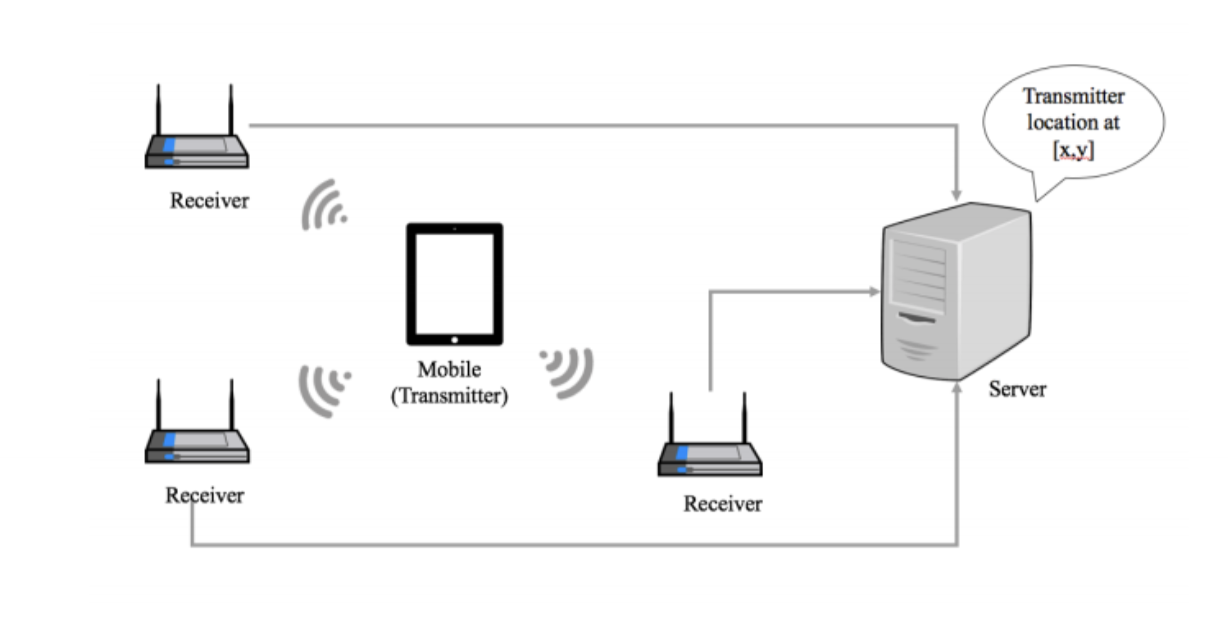
\includegraphics[width=\textwidth]{Image/remotepositioning.png}
\caption{Remote Positioning}
\label{fig:remote}
\end{figure}

\newpage
\subsection{Self Positioning}
\paragraph{}The mobile device will receive the signal from all transmitters. However, the location of all transmitters must be fixed and the mobile device must know where is the all transmitted located. After receiving the signal, the mobile device will act like the center station to calculates its positioning according to the location of transmitters. The overview of self positioning system is show in Figure~\ref{fig:self_positioning}

\begin{figure}[h]
\centering
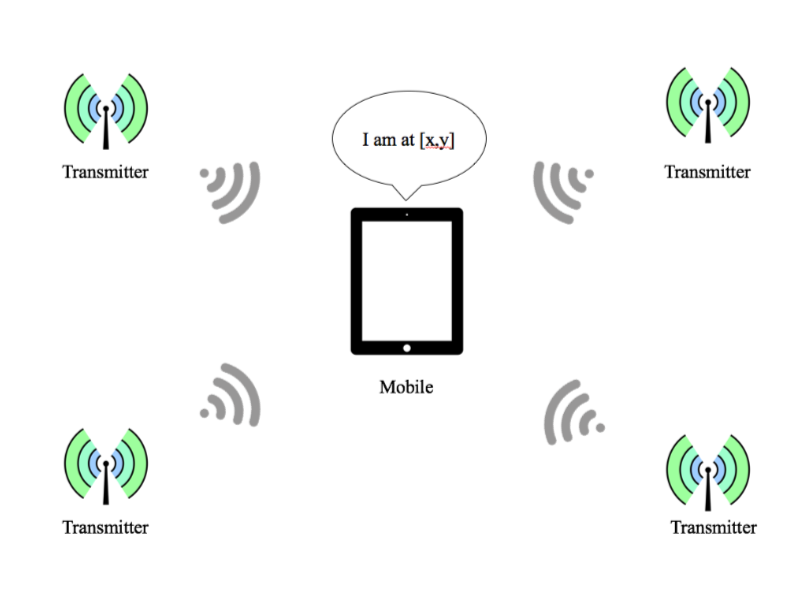
\includegraphics[scale = 0.6]{Image/selfpositioning.png}
\caption{Self Positioning}
\label{fig:self_positioning}
\end{figure}

\newpage
\subsection{Indirect Remote Positioning}
\paragraph{}The mobile device will receive the signal from several transmitters with know the exactly location as same as the self positioning topology. After that the mobile device will calculate the location of itself and send to the remote location. The overview of indirect remote positioning system show in Figure~\ref{fig:indirect_remote}

\begin{figure}[h]
\centering
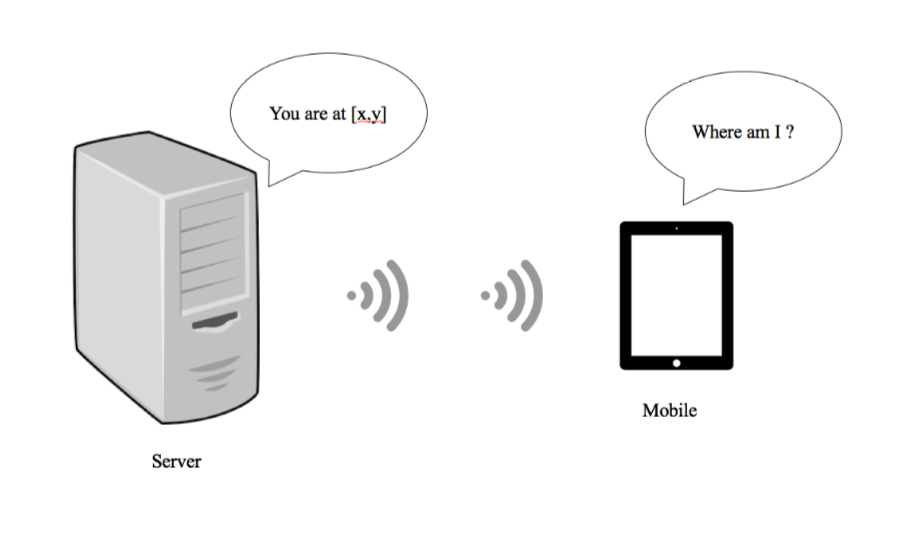
\includegraphics[width=\textwidth]{Image/indirect.png}
\caption{Indirect Remote Positioning}
\label{fig:indirect_remote}
\end{figure}


\newpage
\subsection{Indirect Self Positioning}
\paragraph{} The server collected signal with fixed measuring units from the mobile device. Then the measurement result from the measuring unit will be sent to the mobile device. In short, it is a remote positioning system that transmitting mobile device’s location to the mobile device. Figure~\ref{fig:indirect_self} depicts the overview of indirect self positioning system.

\begin{figure}[h]
\centering
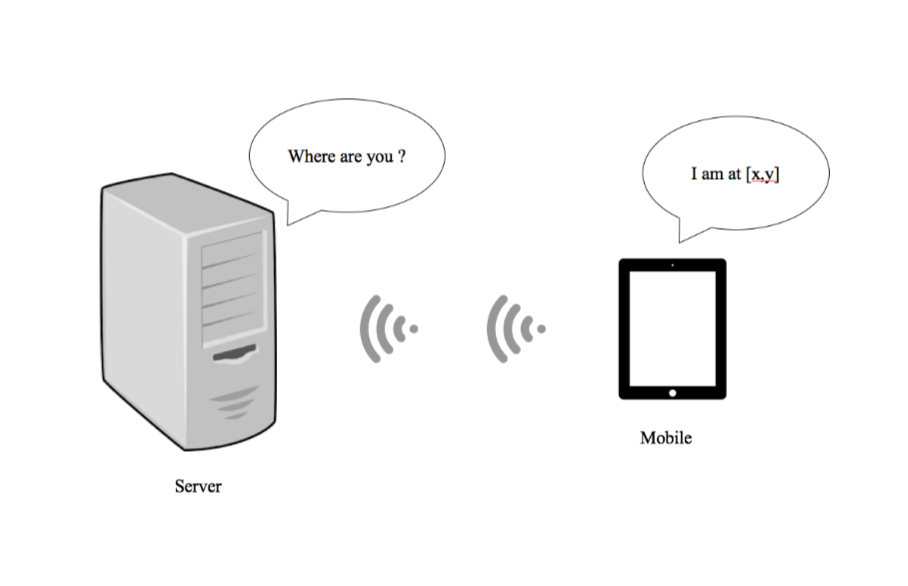
\includegraphics[width=\textwidth]{Image/direct.png}
\caption{Indirect Self Positioning}
\label{fig:indirect_self}
\end{figure}

\newpage
\section{Topology of Outdoor positioning}
\paragraph{}
The Outdoor Positioning Systems could be classified into two categories which
are Global Positioning System (GPS), and cellular network
\subsection{Global Positioning System (GPS)}
\paragraph{}
 GPS is a satellite-based radio-navigation system. It is a global navigation satellite system that provides geolocation and time information to a GPS receiver anywhere on or near the Earth where there is an unobstructed line of sight to four or more GPS satellites. Obstacles such as mountains and buildings block the relatively weak GPS signals. The GPS does not require the user to transmit any data, and it operates independently of any telephonic or internet reception, though these technologies can enhance the usefulness of the GPS positioning information. The GPS provides critical positioning capabilities to military, civil, and commercial users around the world. The United States government created the system, maintains it, and makes it freely accessible to anyone with a GPS receiver.

\subsection{Cellular network}
\paragraph{}
Mobile communication systems such as GSM (Global Standard for Mobile Communications) or UMTS (Universal
Mobile Telecommunication System) are based on a set of cellular networks. Since some years location-based services
(LBS) are delivered by these cellular approaches. LBSs are made possible through a suitable relationship between the
cellular service provider, cellular networks and mobile user’s terminals, which work in synch, to locate the user (mobile
terminal), and then transfer the position data either upon the request or as a continuous stream. The major issue is to
locate the user with a required accuracy and limited latency

\newpage
\section{Positioning Methods}
\paragraph{}
There are many methods have been researched for indoor and outdoor positioning. In this section, it can divided method into three positioning methods;  triangulation, trilateration, and fingerprint-based method. In additional, those locate objects by measuring signals. The main type of signal used in indoor positioning are infrared(IR) and radio frequency(RF) signal and this thesis will focus on using Bluetooth signal which is one type of RF signal.

\subsection{Triangulation}
\paragraph{}Triangulation estimation is a trigonometric approach of determining an unknown location based on two angles and a distance between them. Two or more fixed nodes are required for location estimate by receiving mobile signal (Bluetooth signals) from the signal-transmitting device. Furthermore, angle of Arrival(AoA) is a technique used in triangulation, this technique determines the angle of arrival of the mobile signal sent from the signal-transmitting device at which it is received by multiple receivers. From Figure~\ref{fig:aoa}, the location of the target node T1 is determined by measuring the angles of incidence (q1, q2) at which signals are sent from T1 and arrive at the receiving nodes R1 and R2. Geometric relationships can be used to calculate the coordinate (X,Y) of the target node.
\begin{figure}[h]
\centering
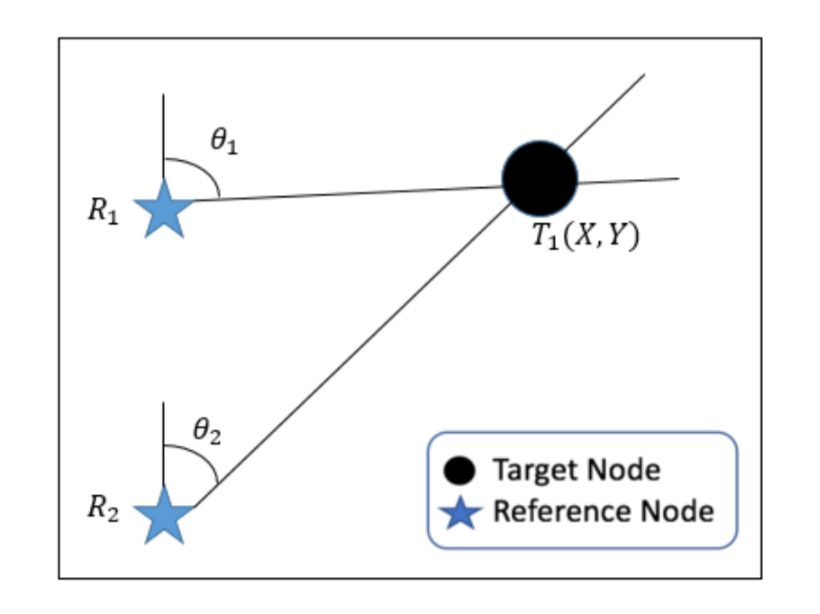
\includegraphics[scale = 0.7]{Image/triangulation.png}
\caption{Angle of Arrival}
\label{fig:aoa}
\end{figure}

\subsection{Trilateration Method}
\paragraph{}Trilateration is a traditional method to compute the unknown position of a node. At least three reference nodes with known positions are required in this method. Besides, the distances between these nodes and the mobile node are required to be known as well. Theoretically, each reference node forms a circle around itself with the radius of the distance to the mobile node. The position of the unknown node corresponds with the intersection of these three circles. Figure~\ref{fig:tri}, where the coordinate of the target object (X,Y) can be estimated using the coordinates of the receivers ((X1,Y1), (X2,Y2) and (X3,Y3)) and the distances (d1, d2 and d3).  Trilateration can be subdivided into two categories namely time-based method and RSSI-based method
\begin{figure}[h]
\centering
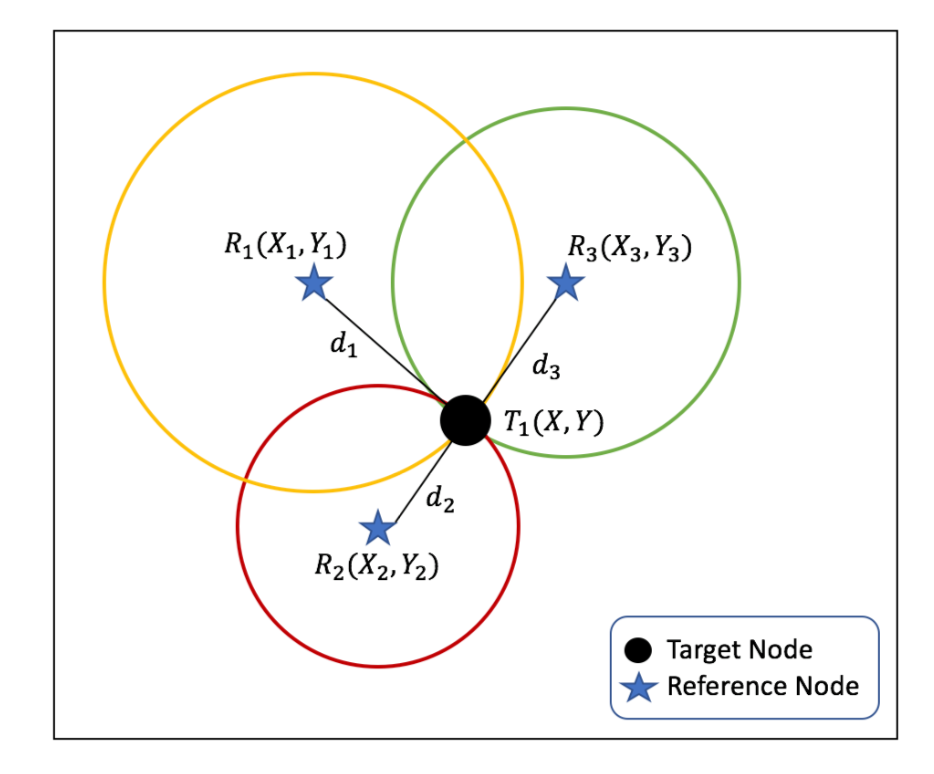
\includegraphics[scale = 0.7]{Image/trileteration.png}
\caption{Trilateration}
\label{fig:tri}
\end{figure}

\newpage
\subsection{Fingerprint-Based Method}
\paragraph{}Fingerprint-Based method is one of the popular techniques for indoor positioning due its high accuracy. The process of the fingerprint method consist of two main phases: training phase and classification phase. During the training phase we have to collect the RSSI data from each room of the target location and map the data into a classification model. After that, we train our system with the model we previously created. Next we go to the classification phase. In this phase the system will receive an input, which will be a RSSI sent from the target object, then it will classify the location of the target object via the model that it had learned. The fingerprint method can be a very accurate method with the use of a massive amount of data in the training phase. With that come a major disadvantage: it requires a lot of set up during the training phase. We need to collect large amount of data in order to just tell what room the device is in. To be able to track the device location with more precision the setup will be too impractical to be beneficial. And also the model that we use to train the system have to be proprietary to each location.



\chapter{Proposed Method}
\section{System Architecture}
\begin{figure}[h]
\centering
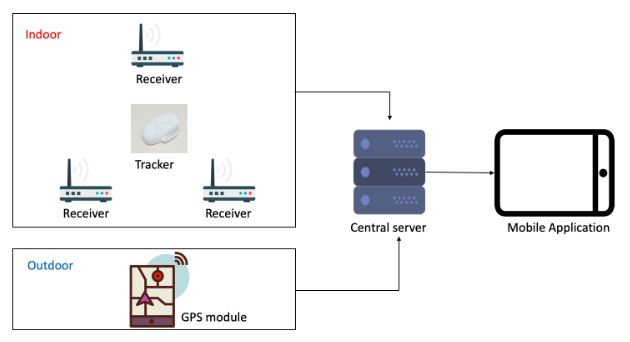
\includegraphics[width=\textwidth]{Image/System_Arch.JPG}
\caption{System Architecture}
\label{fig:system arch}
\end{figure}




\paragraph{}Our research plan to use system architecture shown in Figure~\ref{fig:system arch}. The system contains two main parts: indoor positioning and outdoor positioning. For indoor positioning, the system comprises of three main components: Tracker, Receiver, and Server. Tracker sends Bluetooth signal to the receiver. Then the receiver reads RSSI (Received Signal Strength Indicator) from received signal and sends it to the server. Afterwards, the server preprocesses the RSSI data and then calculate the position of the tracker. The preprocessing techniques used in our research are moving average and channel separation by K-means clustering method. After the data is preprocessed, it is fed into the path loss model in order to obtain the distance between the tracker and the receiver. Lastly, the trilateration method is used to acquire the position of the tracker. The tracker and receiver that we use is BLE (Bluetooth Low Energy) device and Raspberry Pi 3 respectively. The BLE device is used to transmit the Bluetooth signal at the sampling rate of 10 Hertz. The Raspberry Pi 3 is used for receiving the Bluetooth signal from the BLE device in form of RSSI (Received Signal Strength Indication) in decibel unit. Figure~\ref{fig:system arch} shows the devices that we use to collect the RSSI data. For outdoor positioning, the GPS (Global Positioning System) in mobile phone will be enabled when the tracker is no longer in the building, i.e. when the receiver does not receive any signal from the tracker. Figure~\ref{fig:component}a and ~\ref{fig:component}b depict the  device that we use to receiver The RSSI data and Tracker which send the RSSI data respectively  

\begin{figure}[h!]
\centering
\begin{subfigure}[b]{0.4\linewidth}
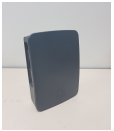
\includegraphics[width=\linewidth]{Image/rasp.png}
\caption{Receiver(RaspberryPi).}
\end{subfigure}
\begin{subfigure}[b]{0.4\linewidth}
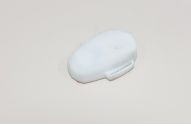
\includegraphics[width=\linewidth]{Image/tracker.png}
\caption{Tracker(Air-Node).}
\end{subfigure}
\caption{Component Deivices.}
\label{fig:component}
\end{figure}


\section{Software Architecture}

\paragraph{}Our software architecture comprises of four components: mobile application for displaying the target object position in 2D map, a cloud-host NoSql database for storing the position of the target object, server for calculating the position of target object, and GPS application for outdoor positioning that will be enabled when the target object is outside of the
building. The server and GPS application send the coordination data to NoSql database. Then the mobile application retrieves that data from database and renders it on 2D map. 
\section{System Process}
\begin{figure}[h]
\centering
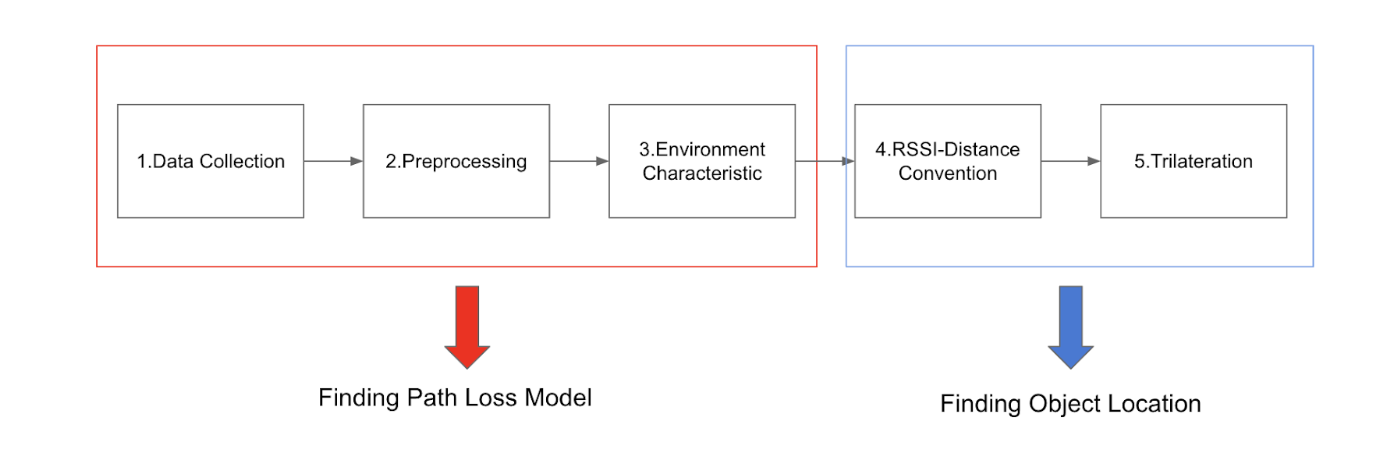
\includegraphics[width=\textwidth]{Image/systemprocess.png}
\label{system_topo}
\caption{System topology}
\end{figure}

\subsection{Data Collection}
\paragraph{}The first process of this section is data collection. In our system, the tracker
attached to the target object send out the Bluetooth signal (BLE). Then the receivers receive the signal from tracker, extract the RSSI data from it, and send that data to the server for further calculation. In the data collection process, the receiver and the tracker are placed on stands with a height of 1 meter. The receiver is placed on a fixed location while the BLE tracker is placed at different distances away from the receiver. At each distance, the tracker is rotated in eight different angles of rotation: 0, 45, 90, 135, 180, 225, 270 and 315 degrees.

\subsection{Preprocess}
\paragraph{}After collecting the raw RSSI data from data collection process, data preprocessing techniques are used for removing unnecessary data and smoothing the noisy data. Two different data preprocessing techniques are applied on the RSSI data of a specific tracker orientation, namely, moving average and channel separation.
\subsubsection{Moving Average}
\paragraph{}Moving average or moving mean is a method to smooth out short-term fluctuations and highlight longer-term trends or cycles by creating series of averages of subset of the whole data set.

\begin{equation}
\centering
y^\prime_1 = \frac{y_1+y_2+y_3+...+y_(w+1)-1}{w}
\label{fig:eqt1}
\end{equation}

\begin{equation}
\centering
y^\prime_2 = \frac{y_2+y_3+y_4+...+y_(w+2)-1}{w} 
\label{fig:eqt1}
\end{equation}

\paragraph{}Where $y^\prime_n$ is the data in the filtered data set, $y_n$ is the data from the original
set and $w$ is the window size. Since we are including the overlapped data, $y_n$will also include the original data at $y_2...y_(w+1)$ - 1in the calculation even though $y_2...y_(w+1) - 1$ is already included in the calculation of Eq. 4.1. After the process is done we will get a filtered data set $y$ which has a significantly less standard deviation than the original data set $y$ .thus, having less noise.

\subsubsection{Chanel Separation}
\paragraph{}The BLE uses three of the 40 channels for broadcasting its advertising packets. The collected data is separated into three clusters for each advertising channel. K-means clustering is performed to distinguish which of the three channels the data belongs to. For each channel, moving average is applied to
smooth the series of data.

\subsection{Environmental Characterization}
\paragraph{}The objective of this method is to find the value of n that constructs a curve that has the lowest total sum of squared error (SSE) or curve fitting process in Eq 4.3, meaning the best fit to the series of data points. SSE measures the deviation between the expected data point and the predicted data point produced by the curve fitting method. After obtaining the result of n, and then use n to substitute in Eq. 4.3 for create Path-loss model.

\begin{equation}
RSSI_d = RSSI_d\textsubscript{0}-10n\log_{10}\frac{d}{d0}
\label{fig:eqt3}
\end{equation}

\paragraph{}In figure\ref{system_topo}, show the example of result after using curve fitting process. Eq. 4.3 forms a curve that best fits this particular set of data points when n is equal to 2.6902 the data is collected in a free space environment. The best fit curve represents the path loss model of the specific environment where the data is collected, the specific angle of the tracker and the specific preprocessing technique performed on the data.
\begin{figure}[h]
\centering
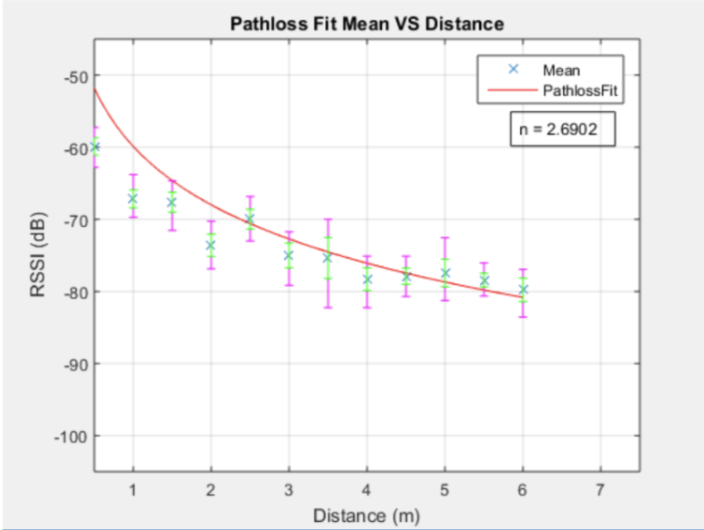
\includegraphics[width=\textwidth]{Image/angle0.png}
\caption{Angle 0, IC 6th floor}
\end{figure}

\newpage
\subsection{RSSI-Distance Conversion(Distance Estimation)}
\paragraph{}In this process, the RSSI value is collected continuously by at least three receivers. The collected RSSI data is preprocessed by the two preprocessing techniques and substituted into the corresponding path loss model to determine the distance between the target object and each receiver. The equation of the path loss model can be rearranged to solve for the distance as in Eq. (4.4).
\begin{equation}
d = d_010\frac{RSSI_d-RSSI_d\textsubscript{0}-X_\sigma}{-10n}
\label{fig:eqt4}
\end{equation}
\paragraph{}The $RSSId_0$ and $n$ is specific to each path loss model (determined in the previous process), while the $RSSI_d$ is obtained from either the mean or median of the preprocessed test set (e.g. mean of data preprocessed by moving average and channel separation, median of data preprocessed by moving median).
\subsection{Trilateration}
\paragraph{}Once we obtain the distances between the target object and each reference node as seen in Figure \ref{fig:self_positioning}, trilateration method can be applied to determine the exact location of the target object. Referring to Figure \ref{fig:tri}, Eq. (4.5), Eq. (4.6) and Eq. (4.7) can be constructed according to the Euclidean distance formula.
\begin{equation}
d_1^2 = (x-x_1)^2+(y - y_1)^2
\end{equation}
\begin{equation}
d_2^2 = (x-x_2)^2+(y - y_3)^2
\end{equation}
\begin{equation}
d_3^2 = (x-x_3)^2+(y - y_3)^2
\end{equation}
\paragraph{}Simplifying the above equations through several mathematical operations produce the following Eq. (4.8) and Eq. (4.9), where Eq. (4.8) is used to find the x coordinate of the target object and Eq. (4.9) is for the y coordinate.
\begin{equation*}
A = -2x_1+ 2x_2
\end{equation*}
\begin{equation*}
B= -2y_1+ 2y_2
\end{equation*}
\begin{equation*}
C = d_1^2- d_1^2-x_1^2+x_2^2-y_1^2+y_2^2
\end{equation*}
\begin{equation*}
D = -2x_2+ 2x_3
\end{equation*}
\begin{equation*}
E = -2x_2+ 2x_3
\end{equation*}
\begin{equation*}
F = d_2^2- d_3^2-x_2^2+x_3^2-y_2^2+y_3^2
\end{equation*}
\begin{equation}
X = \frac{CE-FB}{EA-BD}
\end{equation}
\begin{equation}
X = \frac{CD-AF}{BD-AE}
\end{equation}
\paragraph{}Knowing the coordinates of the three reference nodes (i.e. (x1, y1), (x2, y2), (x3, y3)) and the distances between the target node and the reference nodes (i.e. d1, d2, d3), these known values can be substituted into the equation to obtain the x and y coordinate of the target node.



\chapter{Implementation}
\section{Library}
\subsection{Websockets}
\paragraph{}Websocket is a library for building WebSocket servers and clients in Python with a focus on correctness and simplicity.
\subsection{Bluepy}
\paragraph{}Bluepy is a Python module which allows communication with Bluetooth Low Energy devices.
\subsection{Numpy}
\paragraph{}Numpy is the fundamental package for scientific computing with Python
\subsection{Scipy}
\paragraph{}NumPy is a Python extension module that provides efficient operation on arrays of homogeneous data. It allows python to serve as a high-level language for manipulating numerical data, much like IDL, MATLAB, or Yorick.
\subsection{Sklearn}
\paragraph{}It features various classification, regression and clustering algorithms including support vector machines, random forests, gradient boosting, k-means and DBSCAN, and is designed to interoperate with the Python numerical and scientific libraries NumPy and SciPy.
\section{Development Tools}
\subsection{React native}
\paragraph{}React native is the framework of Javascript that created by Facebook for rendering mobile application. It’s based on React but instead of targeting the browser, it targets mobile platforms React Native uses the same fundamental UI building blocks as regular iOS and Android apps. Therefore, React Native makes it easy to develop and render in both Android and iOS, so it called Cross-platform framework. 
\subsection{Node.js }
\paragraph{}Node.js is the library of Javascript that execute the code outside of a web browser. Usually, JavaScript is used for client-side scripting, in which scripts written in JavaScript are embedded in a webpage's HTML and run client-side by a JavaScript engine in the user's web browser. Node.js lets developers use JavaScript to write command line tools and for server-side scripting, running scripts server-side to produce dynamic web page content before the page is sent to the user's web browser.
\subsection{Firebase Real Time Database}
\paragraph{}Firebase Real Time Database is one of the Firebase's product which provides a realtime database and backend as a service. The service provides application developers an API that allows application data to be synchronized across clients and stored on Firebase's cloud  
\subsection{GitHub}
\paragraph{}GitHub is a web-based version-control and collaboration platform for software developers. GitHub is used to store the source code for a project and track the complete history of all changes to that code. It allows developers to collaborate on a project more effectively by providing tools for managing possibly conflicting changes from multiple developers. 
\subsection{Heroku}
\paragraph{}Heroku is a cloud platform as a service supporting several programming languages such as Java, Node.js, Python, and PHP. Heroku is called a polyglot platform as it has features for a developer to build, run and scale applications in a similar manner across most languages.  
\section{Setup}
\subsection{Pre-processing}
\subsubsection{Moving Average}
\begin{algorithm}
\caption{Moving Average}
\begin{algorithmic}[1]
\Procedure{Moving Average}{$rssi,num$}
\State $m\gets \text{an array with size $rssi$}$
\State $n\gets \text{an array with size $rssi$}$
\State $outFiltered\gets \text{an empty array}$
\For{$i\gets$ 1 to $n$}
    \State $new \gets $rssi$ \text{ start from initial to } i$
    \State $Filtered \gets \text{tsmovavg(new,'s',num,1)} $
    \State $outFiltered \gets \text{an array of outFiltered and Filtered start with num}$
\EndFor
\State $Filtered \gets outFiltered$
\EndProcedure
\end{algorithmic}
\end{algorithm}


\newpage
\subsection{Environmental Characterization}
\begin{algorithm}
\caption{Environmental Characterization}
\begin{algorithmic}[1]
\Procedure{PathLoss}{$dataStat$,$distance$,$statType$}
\State $x-axis\gets \text{list of distance}$
    \If{$checkType(statType, 'Mean' )$}
        \State $dataList \gets \text{use mean value from dataStat}$
    \ElsIf{$checkType(statType, 'Median' )$}
        \State $dataList \gets \text{use mean value from dataStat}$
    \ElsIf{$checkType(statType, 'Mode' )$}
        \State $dataList \gets \text{use mean value from dataStat}$
    \EndIf
\State $ fitType \gets \text{assign path loss model formula}$
\State $[x-data,y-data] \gets \text{assign x-axis data from dataList}$
\State $option \gets \text{set graph mode to non linear graph}$
\State $option-display \gets \text{set to off mode}$
\State $[fitresult,gof] \gets \text{get the result of curve-fitting method}$
\State $n \gets \text{get n value from fitresult}$
\EndProcedure
\end{algorithmic}
\end{algorithm}

\subsection{RSSI-Distance Conversion(DistanceEstimation)}
\begin{algorithm}
\caption{DistanceEstimation}
\begin{algorithmic}[1]
\Procedure{getDistance}{$buffer$,$rssiRefMean$,$nMean$}
\For{each $l$ in enumerate(\text{$kmeans\_model$})}
    \State $rssiMean \gets \text{get mean value from buffer(i)}$
    \State $distanceMean \gets \newline \textss{10^((rssiMean-(rssiRefMean))/(-10^nMean))}$
\EndFor
\State \textbf{return} \text{distanceMean}
\EndProcedure
\end{algorithmic}
\end{algorithm}

\newpage
\subsection{Trilateration}
\begin{algorithm}
\caption{Trilateration}
\begin{algorithmic}[1]
\Procedure{CalculatePosition}{$x_1$,$x_2$,$x_3$,$y_1$,$y_2$,$y_3$,$r1$,$r2$,$r3$}
\State $a\gets \textss{(-2*x1)+(2*x2)}$
\State $b\gets \textss{(-2*y1)+(2*y2)}$
\State $c\gets \textss{(r1)^2+(r2)^2-x_1+x_2-y_1+y_2}$
\State $d\gets \textss{(-2*x_2)+(2*x_3)}$
\State $e\gets \textss{(-2*y_2)+(2*y_3)}$
\State $posX \gets \textss{\frac{(c*e)-(f*b)}{(e*a)-(b*d)}}$
\State $posY \gets \textss{\frac{(c*e)-(a*f)}{(b*d)-(a*e)}}$
\State $position \gets \text{[posX,posY]}$
\State \textbf{return} \text{position}
\EndProcedure
\end{algorithmic}
\end{algorithm}

\section{Proposed System Development}
\paragraph{}The system is developed using mobile application to show the location of both indoor and outdoor positioning in 2-D map.
\subsection{Mobile Application Development}
\paragraph{}To develop the demonstrate mobile application in order to monitor the object position in the indoor and outdoor, we select React Native framework which is created for developing mobile application in both Android and IOS platform. We also use real time database from Firebase that integrated with the application to display all object position in real time. To illustrate more clearly, we choose the hospital’s patient tracking system as a demonstration application. Below are some of the user interface of the mobile application with Figure 5-1 as patients indoor position tracking page. It displays all patients that in the hospital area.

\begin{figure}[h]
\centering
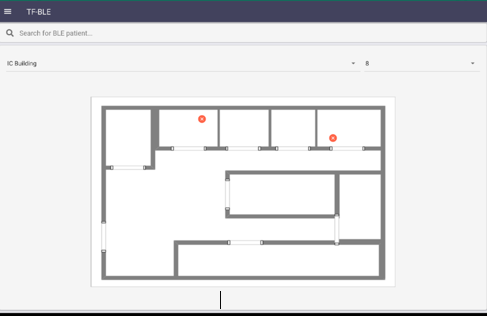
\includegraphics[width=\textwidth]{Image/bright1.png}
\caption{}
\label{bright1}
\end{figure}

\newpage
\paragraph{}In additional, it can track a wanted patient by press a search bar from Figure \ref{bright1} and then it will show the list of patients in Figure \ref{bright2}. Admin can input the word to filter the list and select patient and then it will display in Figure \ref{bright3}

\begin{figure}[h]
\centering
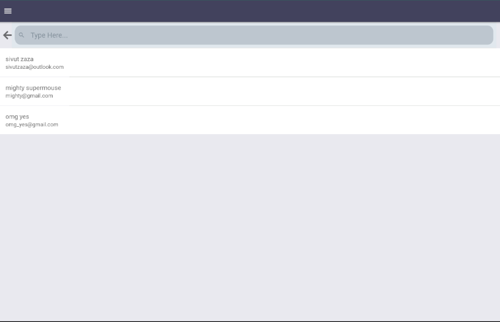
\includegraphics[width=\textwidth]{Image/bright2.png}
\caption{}
\label{bright2}
\end{figure}

\begin{figure}[h]
\centering
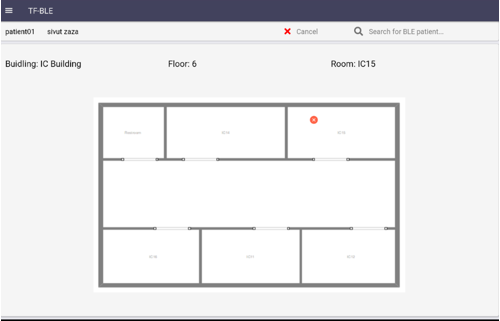
\includegraphics[width=\textwidth]{Image/bright3.png}
\caption{}
\label{bright3}
\end{figure}

\newpage
\newpage
In outdoor position tracking page, it works same as an indoor position page. It displays all patients that already outside the hospital area. Below are some of the user interface of the outdoor position tracking page as Figure \ref{bright4} . Moreover, it can track wanted patient by press a search bar in Figure \ref{bright4} and then it will show the lists of outside patients same as indoor positioning mode in Figure \ref{bright2}. After select wanted patient, it will display in Figure \ref{bright5}     
    

\begin{figure}[h]
\centering
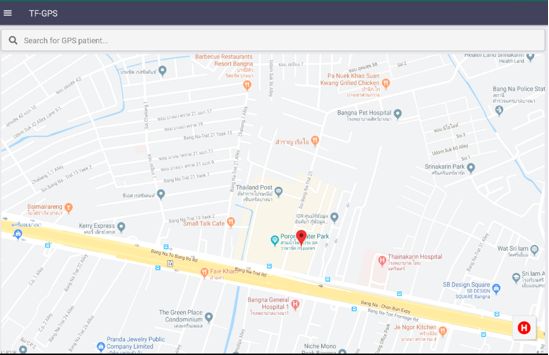
\includegraphics[width=\textwidth]{Image/bright4.png}
\caption{}
\label{bright4}
\end{figure}



\begin{figure}[h]
\centering
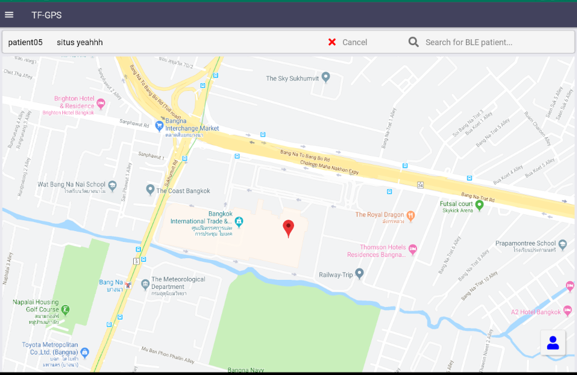
\includegraphics[width=\textwidth]{Image/bright5.png}
\caption{}
\label{bright5}
\end{figure}


\chapter{Experiment \& Result}
This chapter explains experiment setup and showing the result for all process from the proposed method in the chapter 4. In additional, each process has to full fill its own objectives as well as satisfy the objective of this thesis overall. 
\section{Dataset}
All dataset in our experiment are collected in an open area with no obstacle between tracker and receiver inside the 6th floor of the International College building in King Mongkut’s Institute of Technology Ladkrabang (KMITL) at eight different angle of rotations of the tracker: angle 0, angle 45, angle 90, angle 135, angle 180, angle 225, angle 270, and angle 315.\\
\\
\noindent \textbf{Training Sets}
\newline Following is the list of all datasets we collected using Raspberry Pi 3 Receive and BLE tracker.
\begin{enumerate}
    \item Dataset 1: 200 samples at 12 distances, 0.5, 1, 1.5, 2, 2.5, 3, 3.5, 4, 4.5, 5, 5.5, and 6 meters collected on October 17, 2018.
    \item Dataset 2: 200 samples at 12 distances, 0.5, 1, 1.5, 2, 2.5, 3, 3.5, 4, 4.5, 5, 5.5, and 6 meters collected on November 12, 2018.
    \item Dataset 3: 200 samples at 12 distances, 0.5, 1, 1.5, 2, 2.5, 3, 3.5, 4, 4.5, 5, 5.5, and 6 meters collected on November 21, 2018.
    \item Dataset 4: 200 samples at 12 distances, 0.5, 1, 1.5, 2, 2.5, 3, 3.5, 4, 4.5, 5, 5.5, and 6 meters collected on December 04, 2018.
    \item Dataset 5: 200 samples at 12 distances, 0.5, 1, 1.5, 2, 2.5, 3, 3.5, 4, 4.5, 5, 5.5, and 6 meters collected on February 20, 2019.
    \item Dataset 6: 200 samples at 12 distances, 0.5, 1, 1.5, 2, 2.5, 3, 3.5, 4, 4.5, 5, 5.5, and 6 meters collected on March 1, 2019.
\end{enumerate}
\section{Measure}
\subsection{Root Mean Squared Eror(RMSE)}
The statistical measures that we use to evaluate the performance of our
system are the minimum absolute error, maximum absolute error, standard deviation of the absolute errors and the Root Mean Squared Error (RMSE). The
absolute error measures the absolute difference between the expected and the
actual result. RMSE basically measures the average of the differences between
the expected and the actual results, calculated by Eq \ref{RMSE}
\begin{equation}
RMSE = \sqrt{\frac{1}{n} \sum_{i=1}^{n} (y_i-\hat{y_i})^2}
\label{RMSE}
\end{equation}
where $n$ is the number of predictions, $y$ is the vector of expected values and $\hat{y}$ is the vector of actual values being predicted.
\subsection{Precision Score}
The precision score is ratio of correctness,it is a metric for multi-label classification of how many selected items are relevant
\begin{equation}
Precision Score = \frac{TP}{TP+FP}
\label{precision}
\end{equation}
where $tp$ is the number of true positives and $fp$ the number of false positives. The precision is intuitively the ability of the classifier not to label as positive a sample that is negative.
The best value is 1 and the worst value is 0.


\section{Experiment}
There are four experiments on all of our datasets to study the nature of the data and formulate hypotheses. In this section, the author explore the factors that related to the performance of the system. It consist of Preprocessing technique, and environment variable in Path loss model. 
\subsection{Experiment1: Preprocessing by Moving Average}
\subsection*{Objective}
\noindent This experiment explains the effectiveness of RSSI after reducing the noise of data by using moving average and visualize the path loss model from the moving average of RSSI data.


\subsection*{Experimental Procedure}
The raw RSSI set is filtered by moving average with a windows size of 20, using Matlab on test set for all 8 angles of vertical rotation to smooth the RSSI readings before the curve fitting is performed on the means of the filtered data to obtain the
path loss model

\begin{figure}[H]
\centering
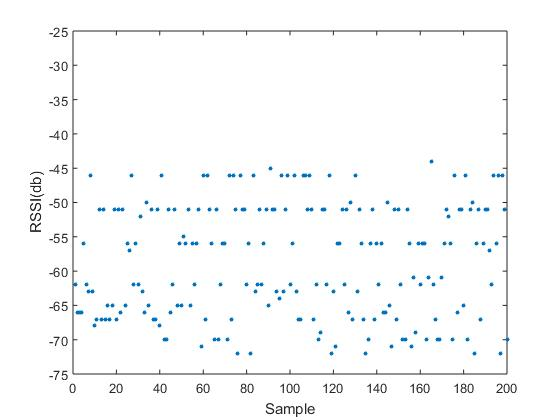
\includegraphics[width=\textwidth]{Image/scatterRaw.jpg}
\caption{Scatter plot of raw data}
\label{}
\end{figure}


\begin{figure}[H]
\centering
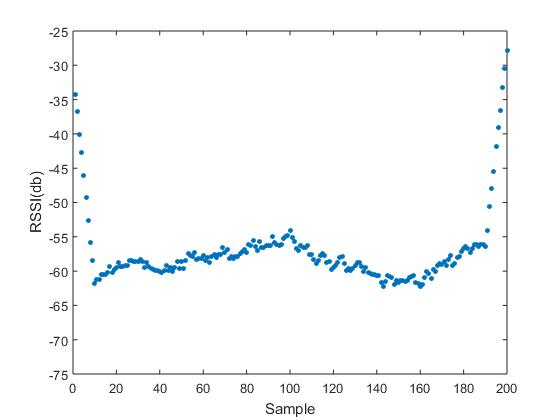
\includegraphics[width=\textwidth]{Image/s05Avg.jpg}
\caption{Scatter plot of data after applying moving average}
\label{}
\end{figure}



\subsection*{Result}
The data is less scatter and smoother after applying the moving average. The data before applying the moving average is shown in Fig.6.1 and the data after applying the moving average is shown in Fig.6.2.

\begin{figure}[H]
\centering
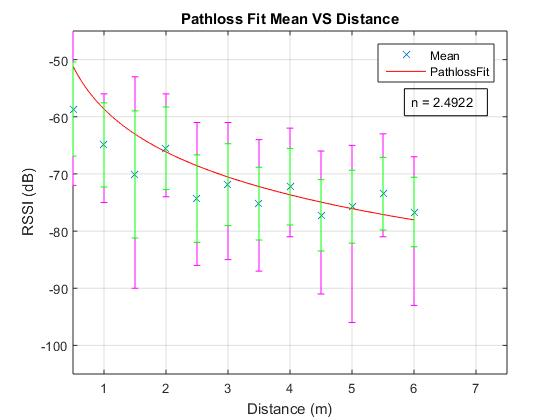
\includegraphics[width=\textwidth]{Image/rawCurveFit0.jpg}
\caption{Curve fitting of raw data at angle 0}
\label{}
\end{figure}

Fig.6.3 shows the result of curve fitting to pathloss model of raw data at angle 0. The pink bar at each point indicates its min-max error bar, while the green bar indicates its standard deviation.

\begin{figure}[H]
\centering
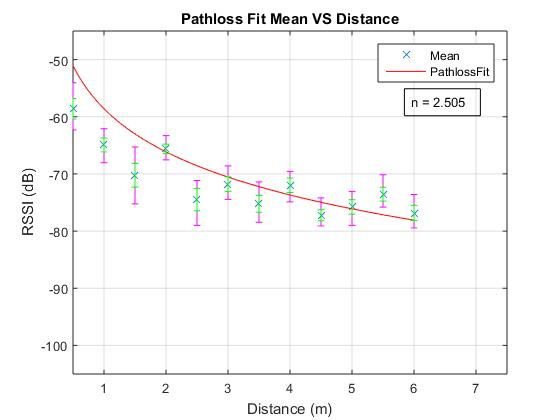
\includegraphics[width=\textwidth]{Image/curveFit0.jpg}
\caption{Curve fitting of data at angle 0 after applying moving average}
\label{}
\end{figure}

Fig.6.4 shows the result of curve fitting to pathloss model of the data at angle 0 after filtering with moving average. From the observation, the min-max error bar and the standard deviation in Fig.6.4 is significantly smaller comparing to the plot shown in Fig.6.3. The conclusion of statistics from before applying filter and after applying filter is shown in Fig.6.5 and Fig.6.6 respectively.

\begin{figure}[H]
\centering
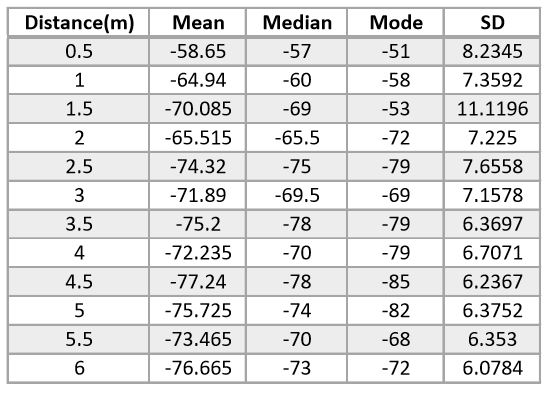
\includegraphics[width=\textwidth]{Image/rawTable.JPG}
\caption{Statistics details of raw data at angle 0}
\label{}
\end{figure}

\begin{figure}[H]
\centering
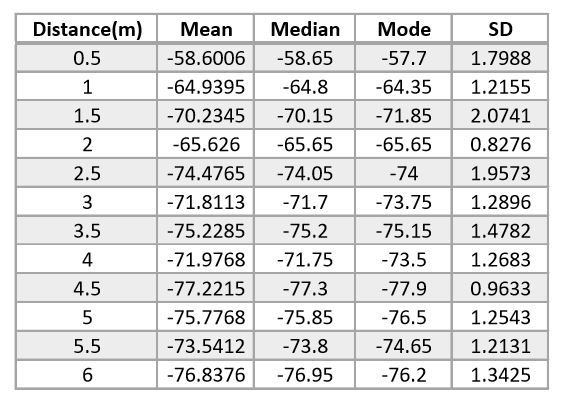
\includegraphics[width=\textwidth]{Image/movAvgTable.JPG}
\caption{Statistics of data at angle 0 after applying moving average filter}
\label{}
\end{figure}



\subsection{Experiment2: Prediction of $n$ variable in Path Loss Model}
\subsection*{Objective}
This experiment is conducted in an attempt to predict the $n$ variable which is the environment variable that can directly affect to the accuracy of RSSI-Distance Conversion (Distance Estimation) in Eq. (4.4)
\subsection*{Experimental Procedure}
The curve fitting to pathloss model is performed on filtered RSSI data. After the curve fitting process and the $n$ variable is obtained, we to plot the value of $n$ from we retrieved from curve fitting at every angles and observe the trend of the graph.

\begin{figure}[H]
\centering
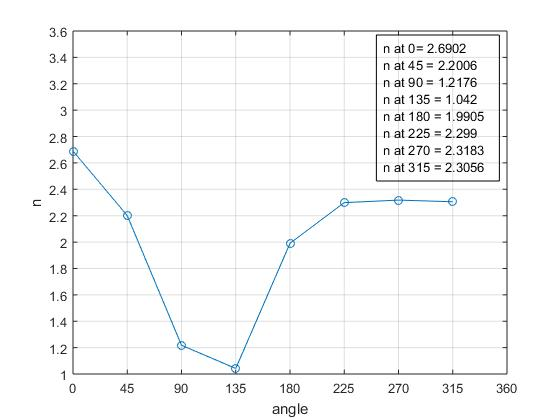
\includegraphics[width=\textwidth]{Image/pltN1.jpg}
\caption{Plot of $n$ from Dataset 1}
\label{}
\end{figure}

\begin{figure}[H]
\centering
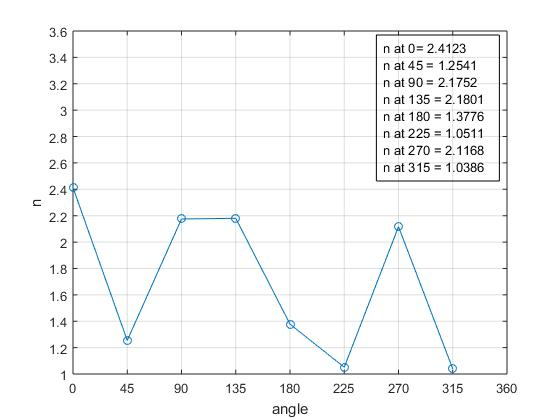
\includegraphics[width=\textwidth]{Image/pltN2.jpg}
\caption{Plot of $n$ values from Dataset 2}
\label{}
\end{figure}

\begin{figure}[H]
\centering
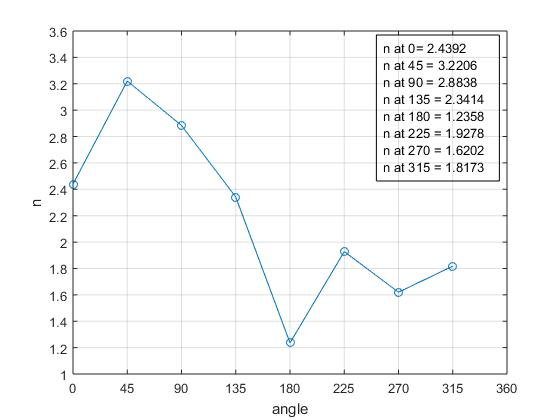
\includegraphics[width=\textwidth]{Image/pltN3.jpg}
\caption{Plot of $n$ values from Dataset 3}
\label{}
\end{figure}

\begin{figure}[H]
\centering
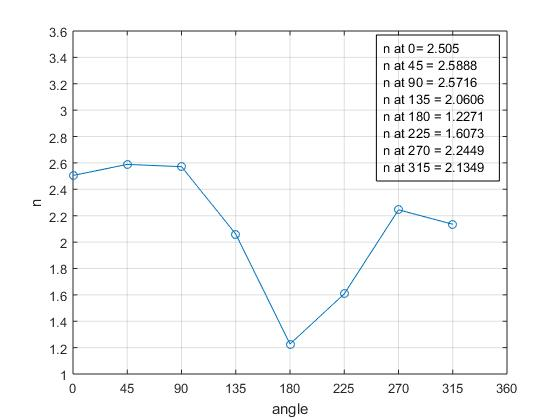
\includegraphics[width=\textwidth]{Image/pltN4.jpg}
\caption{Plot of $n$ values from Dataset 4}
\label{}
\end{figure}

\subsection*{Result}
We did this experiment in hope to be able to determine the pattern of the graph by observing each plot. However, unfortunately, the pattern that we get from each dataset varies too much to be able to infer the overall pattern. For example, the pattern from Fig.6.8 is similar to the graph of sine, though, the same cannot be said for the rest. The pattern from Fig.6.9 and Fig.6.10 is similar to each other as their RSSI data were collected on the same date and almost at the same time. Nevertheless, there is an inadequate information to conclude the pattern according to the graph trend.

\subsection{Experiment 3: Trilateration}
\subsection*{Objective}
This experiment is conducted to evaluate the performance of trilateration by the
path loss models of known angle (angle 0) obtained from preprocessing techniques: moving average with window size of 20
separation technique
\subsection*{Experimental Procedure}
Our training set consists of the RSSI data of angle 0 from Dataset 5.
It is preprocessed by applying a moving average filter and then curve fitted
to obtain the pathloss models. 

For the test set, we use the 200 samples of RSSI data that are collected real-time
by each receiver. Similar to the training set, it is preprocessed by applying the 
moving average filter and curve fitted into the pathloss models to estimate
the distance between the target object and the receiver before applying the trilateration
technique to acquire the position of the target object. The three closest
receivers based on the distance between receiver and tracker(target object) will be
used for the trilateration. Figure \ref{fig:tri_setup} and \ref{fig:realtri_setup} show the setup of receiver and tracker
for the trilateration experiment.

\begin{figure}
\centering
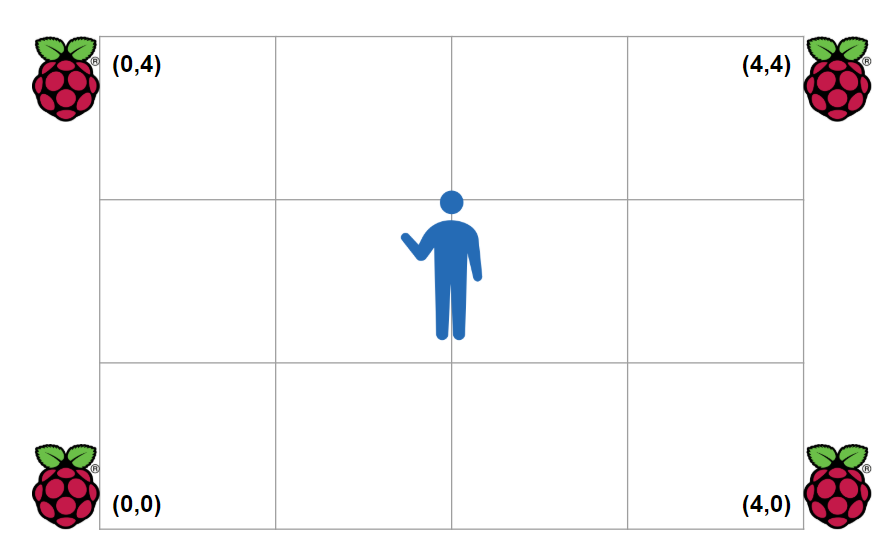
\includegraphics[width=\textwidth]{Image/area.png}
\caption{Overview of Trilateration Setup}
\label{fig:tri_setup}
\end{figure}

\begin{figure}
\centering
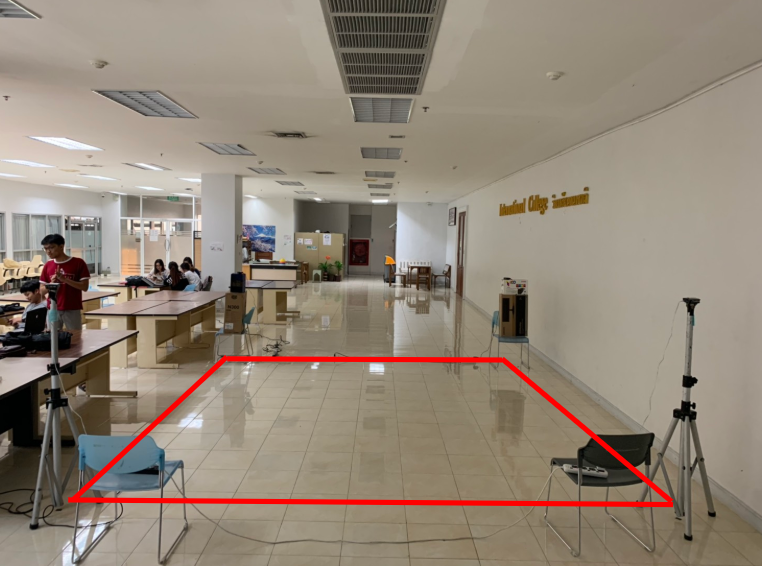
\includegraphics[width=\textwidth]{Image/realarea.png}
\caption{Trilateration Setup on 6th Floor of IC KMTL }
\label{fig:realtri_setup}
\end{figure}

\newpage
\subsection*{Result}
From the table, it show the performance comparison of trilateration at different position based on Root Mean Square Error(RMSE), minimum absolute error, maximum absolute error and the standard deviation (SD) of the absolute errors. In RMSE the value that close to 0 that mean no error occur. However, it can see that the minimum and maximum, of RMSE are 0.62 and 1.19 respectively, it can conclude that are very high RMSE and illustrate there are a huge error on this experiment.
\begin{table}[]
\begin{tabular}{|l|l|l|l|l|l|l|}
\hline
                           & \multicolumn{1}{c|}{(0,0)} & \multicolumn{1}{c|}{(1,0)} & (2,1) & (3,3) & (0,4) & (4,4) \\ \hline
\multicolumn{1}{|c|}{RMSE} & 0.86                       & 1.19                       & 0.62  & 0.82  & 0.83  & 1.1   \\ \hline
Min Abs Error              & 0.14                       & 0.04                       & 0.48  & 0.16  & 0.13  & 0.14  \\ \hline
Max Abs Error              & 2.40                       & 2.6                        & 3.1   & 2.56  & 1.7   & 4.25  \\ \hline
\multicolumn{1}{|c|}{SD}   & 0.71                       & 0.77                       & 0.89  & 0.64  & 0.52  & 1.16  \\ \hline
\end{tabular}
\caption{Statistics of trilateration result}
\label{result_rmse}
\end{table}

\newpage
\subsection{Experiment 4: Trilateration with logic condition}
\subsection*{Objective}
This experiment tired to reduce the error in RMSE from Experiment 3 by setting logic condition rule to avoid the fluctuate result which product from tracker
\subsection*{Experimental Procedure}
Due to the high error of RMSE that show in Experiment 3, this experiment tried to reduce error by making logic condition. From \ref{diagram_logic}, it can be obviously seen that after trilateration computing to get the coordinate position of object ex (1,3), it will sent this value to logic condition process to compute. After that,system will get the result. Figure \ref{logicalgo} it demonstrate the result from logic condition when position of object is inside the range of that are set. For instance, if the position of object is (1,1.5) after pass to logic condition, the result will be "Block1"

\begin{figure}[h]
\centering
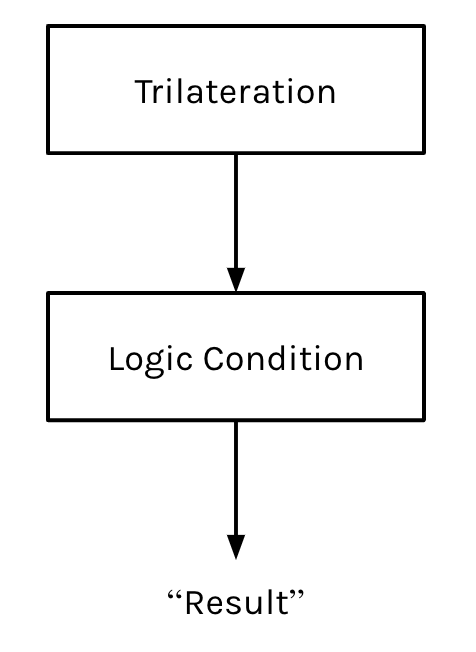
\includegraphics[width={0.4\textwidth}]{Image/diagram_logic2.png}
\caption{}
\label{diagram_logic}
\end{figure}

\begin{figure}[h]
\centering
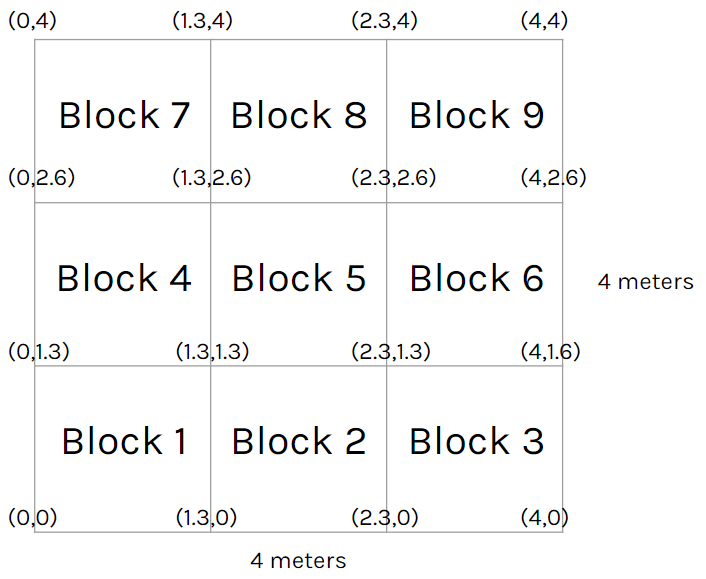
\includegraphics[width={\textwidth}]{Image/blog33.png}
\caption{}
\label{logicalgo}
\end{figure}



\newpage
\subsection{Result}
From table \ref{result_rmse2}, it show the precision score of trilateration with logic condition,the highest precision score is 0.88 at block9 and lowest score is 0.77. Moreover, the standard deviation is 0.053 that means that the result do not have a lot of “spread”. The result in the sample don't vary much, and are very tightly clustered together.
\newline
\begin{sidewaystable}[]
\begin{tabular}{|l|l|l|l|l|l|l|l|l|l|}
\hline
                                                                                         & Block1 & Block2 & Block3 & Block4 & Block5 & Block6 & Block7 & Block8 & Block9 \\ \hline
Precision Score                                                                          & 0.91   & 0.69   & 0.91   & 0.60   & 0.47   & 0.65   & 0.91   & 0.52   & 0.91   \\ \hline
\multicolumn{1}{|c|}{\begin{tabular}[c]{@{}c@{}}Average \\ Precision Score\end{tabular}} & \multicolumn{9}{c|}{0.73}                                                     \\ \hline
\multicolumn{1}{|c|}{SD}                                                                 & \multicolumn{9}{c|}{0.17}                                                     \\ \hline
\end{tabular}

\caption{Statistics of trilateration with logic condition result}
\label{result_rmse2}
\end{sidewaystable}

\chapter{Conclusion}
\paragraph{}In this thesis, the objectives are to improve the BLE indoor positioning and implement a mobile application that display the indoor and outdoor location of the object in 2-D map. It contributes to the study and research of the nature of n variable which directly affects the performance of the system. In addition, the authors collect RAW data of RSSI in multiple sets in several environments to see the trend and predict the n value in real-time. Unfortunately, there are many factors that are related to n variable such as, interference of signal, temperature, etc. Thus, the value cannot be predicted. However, to achieve our objective, the authors set a logical condition after trilateration process to get the position and return a more reliability result. From the result, the authors can achieve a high precision score of 0.88 and  standard deviation of 0.053.
\section{Problem and Obstacle}
\paragraph{}
\subsection{Hardware Limitation}
\paragraph{}For Bluetooth Low Energy device 4.1, the  RSSI value send from the device is very fluctuate and unreliable in sometimes. Especially, the environmental factors such as objects or people in the area could  affect the BLE signal transmission which also leads to wrong distances estimation.

\section{Future work}
\subsection{Hardware}
\paragraph{}In the future, there will be Bluetooth 5.1 which has direction-finding feature that will let Bluetooth devices pinpoint physical location to the centimeter, aiding in indoor positioning. Bluetooth 5.1 offers two different methods for determining direction, named “Angle of Arrival” (AoA) and “Angle of Departure” (AoD). One of the two devices must have an array of multiple antennas, and the data received from those antennas can be used to identify the direction the Bluetooth signal is coming from.
\paragraph{}If you’re carrying a smartphone around and that phone has Bluetooth 5.1, a positioning system can have a good idea about your exact location. This could be used to improve navigation indoors, find your lost keys, or enable smarthome hardware to better pinpoint your location
\subsection{Algorithm}
\paragraph{}In indoor positioning computation method, there are many solutions to improve the positioning performance For example, Indoor Positioning System with Pedestrian Dead Reckoning and BLE Inverse Fingerprinting by H. J. Bae and L. Choi [24]
\renewcommand{\bibname}{References}

\begin{thebibliography}{2}

\bibitem{ref:r1}
Z. C. Jean et al. A 10-gram microflyer for vision-based indoor navigation. In 2006 IEEE/RSJ International Conference on Intelligent Robots and Systems, pages 3267–3272, 2006.
\bibitem{ref:r2}
A. Abdulrahman et al. Ultra wideband indoor positioning technologies: Analysis and recent advances. Sensors (Basel), 16, 2016.
\bibitem{ref:r3}
C. Chanaphon and P. Punyanuch. Camfinder: Image-Based Indoor Positioning System.PhD thesis, King Mongkut’s Institute of Technology Ladkrabang, 2014.
\bibitem{ref:r4}
H. Andy et al. The anatomy of a context-aware application. 8:187–197, 2002.
\bibitem{ref:r5}
W. Roy. An introduction to rfid technology. IEEE Pervasive Computing, 5:25–33, 2006.
\bibitem{ref:r6}
Chunhan Lee, Yushin Chang, Gunhong Park. Indoor positioning system based on incident angles of infrared emitters. Industrial Electronics Society, 2004. IECON 2004
\bibitem{ref:r7}
M. K. Mohamed, P. Sourav, and L. Alexander. Designing simple indoor navigation system for uavs. In 2011 19th Mediterranean Conference on Control and Automation (MED), pages 1223–1228, 2011
\bibitem{ref:r8}
SEBASTIAN DÄDEBY JOAKIM HESSELGREN. A system for indoor positioning using ultra-wideband technology. Department of Computer Science and Engineering CHALMERS UNIVERSITY OF TECHNOLOGY UNIVERSITY OF GOTHENBURG Gothenburg, Sweden 2017
\bibitem{ref:r9}
Chanatip C, Chawin T, Suppakorn S, Isara A. A Pre-processing Technique for BLE-based Indoor Localization. King Mongkut’s Institute of Technology Ladkrabang	Bangkok, Thailand 2018
\bibitem{ref:r10}
Shinsuke Kajioka, Tomoya Mori, Takahiro Uchiya, Ichi Takumi and Hiroshi Matsuo, "Experiment of Indoor Position Presumption Based on RSSI of Bluetooth LE Beacon," IEEE 3rd Global Conference on Consumer Electronics (GCCE), 2014.
\bibitem{ref:r11}
J. N. S. C. Hyunwook Park, "Three-dimensional positioning system using Bluetooth low-energy beacons," International Journal of Distributed, vol. 12(10), 2016. 
\bibitem{ref:r12}
R. H. Ramsey Faragher, "Location Fingerprinting With Bluetooth Low Energy Beacons," IEEE Journal on Selected Areas in Communications, vol. 13, no. 11, pp. 2418-2428, 2015.
\bibitem{ref:r13}
A. D. Blas and D. López-de-Ipiña, "Improving trilateration for indoors localization using BLE beacons," 2017 2nd International Multidisciplinary Conference on Computer and Energy Science (SpliTech), 2017.
\bibitem{ref:r14}
G. Yanying and L. Anthony. A survey of indoor positioning systems for wireless personal networks. IEEE Communications Surveys and Tutorials, 11:13–32, 2009.
\bibitem{ref:r15}
C. David, C. Mario, and S. David de la Torre. Performance evaluation of bluetooth low energy in indoor positioning systems. Trans. Emerging Telecommunications Technologies, 25:1–10, 2014.
\bibitem{ref:r16}
J. Zhu et al. Rssi based bluetooth low energy indoor positioning. In 2014 International Conference on Indoor Positioning and Indoor Navigation (IPIN), pages 526–533, 2014.
\bibitem{ref:r17}
 F. Ramsey and H. Robert. Location fingerprinting with bluetooth low energy beacons. IEEE Journal on Selected Areas in Communications, 33, 2015.
\bibitem{ref:r18}
L. Hui, D. Houshang, B. Pat, and L. Jing. Survey of wireless indoor positioning techniques and systems. IEEE Transactions on Systems, Man, and Cybernetics, 37:1067–1078, 2007.
\bibitem{ref:r19}
C. Chanaphon and P. Punyanuch. Camfinder: Image-Based Indoor Positioning System. PhD thesis, King Mongkut’s Institute of Technology Ladkrabang, 2014.
\bibitem{ref:r20}
C. Panarat and S. D. Joko. Indoor localization system using wireless sensor networks for stationary and moving target. In 2011 8th International Conference on Information, Communications and Signal Processing, 2011.
\bibitem{ref:r21}
H. W. Fentaw and T. Kim, "Indoor localization using magnetic field anomalies and inertial measurement units based on Monte Carlo localization," 2017 Ninth International Conference on Ubiquitous and Future Networks (ICUFN), 2017.
\bibitem{ref:r22}
Navigation National Coordination Office for Space-Based Positioning and Timing. Gps accuracy, August 2017.
\bibitem{ref:r23}
R. Faragher, R. HarleAn. Analysis of the Accuracy of Bluetooth Low Energy for Indoor Positioning Applications.

\bibitem{ref:r24}
H. J. Bae and L. Choi, Indoor Positioning System with Pedestrian Dead Reckoning and BLE Inverse Fingerprinting, November 2018

\end{thebibliography}

\end{document}
